\chapter{Интегральная формула Коши. Разложение функции, регулярной в окрестности точки, в ряд Тейлора.}
\section{Интегральная формула Коши}

\begin{exmpl}
\label{exmpl1}
Вычислить интеграл 
$$
I_k = \int_{\gamma_r} (z-a)^k\,dz, \quad k \in \bbZ, \; a\in \bbC
$$
где контур $\gamma_r$ есть окружность $\{ z \bigl|\bigr. |z - a| = r>0 \}$,ориентированная движением против хода часовой стрелки.
\end{exmpl}
\begin{solution}
Выберем параметризацию окруности $\gamma_r$ вида $z = a + r e^{i \varphi}$, где $\varphi \in [0, 2\pi]$. Тогда

$$
I_k = \int_{0}^{2 \pi} r^k e^{i k \varphi} r i e^{i \varphi} \,d\varphi = i r^{k+1} \int_{0}^{2 \pi} e^{i (k + 1) \varphi}\,d\varphi.
$$

В Итоге
\begin{enumerate}
\item
При $k = -1$ получаем $J_{-1} = i \int_{0}^{2\pi}\,d\varphi = 2 \pi i$;
\item
При $k \ne -1$ получаем
$
J_k = i r^{k + 1} \left( \int_{0}^{2 \pi} cos(k + 1) \varphi \,d \varphi + i \int_{0}^{2 \pi} sin(k + 1) \varphi \,d\varphi \right) = 0.
$
\end{enumerate}
\end{solution}

\begin{thm} \label{ch34thm1}

 Пусть $G$ --- ограниченная область в $\bbC$ с кусочно-гладкой положительно ориентированной границей $\Gamma$. Пусть функция $f\colon \overline{G}\to \bbC$ регулярна на $G$ и непрерывна на $G=G\cup\Gamma$. Тогда для любой точки $z\in G$ справедлива интегральная формула Коши вида
 
 \begin{equation} \label{ch34eq1}
 f(z) = \frac{1}{2\pi i}\int_\Gamma \frac{f(\zeta)}{\zeta - z}\,d\zeta.
 \end{equation}
\end{thm}
\begin{proof}
Фиксируем произвольную точку $z \in G$. Функция $\frac{f(\zeta)}{\zeta - z}$ регулярна по переменному $\zeta$ в области $G \setminus \{z\}$. Выберем число $r_0 > 0$ такое, что выполнено включение $\overline{B_{r_0}(z)}\subset G$. 

\addpicture{pictures/ch34pict1}{0.5}\label{ch34pict1} Обозначим через $\gamma \triangleq \{ \zeta \bigl| |\zeta - z| = r \}$ окружность радиуса $r \in (0, r_0)$ ориентированную против хода часовой стрелки. Обозначим множества $G_r \triangleq G \setminus \overline{B_r(z)}$ и $\Gamma_r \triangleq \Gamma \cup \gamma_r^{-1}$. Очевидно, что множество $G_r$ есть область с кусочно-гладкой положительно ориентированной границей $\Gamma_r$(рис.\ref{ch34pict1}). 

По обощенной интегральной теореме Коши \ref{abc28} из билета №33 получаем

 \begin{equation} \label{ch34eq2}
 0 = \int_{\Gamma_r} \frac{f(\zeta)}{\zeta - z}\,d\zeta = \int_\Gamma \frac{f(\zeta)}{\zeta - z}\,d\zeta - \int_{\gamma_r} \frac{f(\zeta)}{\zeta - z}\,d\zeta.
 \end{equation}
Итак,

\begin{equation} \label{ch34eq3}
J \triangleq \frac{1}{2\pi i} \int_\Gamma \frac{f(\zeta)}{\zeta - z}\,d\zeta \myeq{\eqref{ch34eq2}} \frac{1}{2\pi i} \int_{\gamma_r} \frac{f(\zeta)}{\zeta - z}\,d\zeta,  \quad  \forall r: 0 < r < r_0
\end{equation}

Как показано в примере \ref{exmpl1}, справедливо равенство $1 = \frac{1}{2\pi i} \int_{\gamma_r} \frac{1}{\zeta - z}\,d\zeta$, откуда 

$$J - f(z) = \frac{1}{2\pi i} \int_{\gamma_r} \frac{f(\zeta) - f(z)}{\zeta - z}\,d\zeta, \quad  \forall r \in (0,r_0)$$

Так как $f(\zeta)$ непрерывна в точке $z \in G$, то для каждого $\epsilon > 0$ существует $\delta(\epsilon) \in (0, r_0)$ такое, что $\forall \zeta : |\zeta - z| < \delta(\epsilon)$ следует $|f(\zeta) - f(z)| < \epsilon$. Поэтому выбирая $r \in (0, \delta(\epsilon))$, получаем

\begin{equation} \label{ch34eq4}
|J - f(z)| \le \frac{1}{2\pi} \int_{\gamma_r} \frac{|f(\zeta) - f(z)|}{|\zeta - z|}|\,d\zeta| \le 
\frac{\epsilon}{2 \pi r} \int_{\gamma_r} |\,d\zeta| = \epsilon.
\end{equation}

Так как $\epsilon > 0$ произвольное число, то из (3), (4) следует $J = f(z)$, т.е. формула $\eqref{ch34eq1}$.
\end{proof}

\begin{defn}\label{ch34defn1}
Пусть $\gamma$ — кусочно-гладкий контур в $\bbC$ и пусть $\omega = q(z)$ — непрерывная на $\gamma$ функция. Тогда интеграл вида

\begin{equation} \label{ch34eq5}
I(z) \triangleq \frac{1}{2 \pi i} \int_\gamma \frac{q(\zeta)}{\zeta - z}\,d\zeta, \quad z \notin \gamma
\end{equation}
называется интегралом типа Коши по контуру $\gamma$ от функции $q$.
\end{defn}

\begin{thm} \label{ch34Thm2}
При сформулированных в определении \ref{ch34defn1} условиях функция $I:\bbC \setminus \gamma \to \bbC$ из $\eqref{ch34eq5}$ определена и дифференцируема бесконечное число раз, причем для производных справедлива формула

\begin{equation} \label{ch34eq6}
I^{(n)}(z) = \frac{n!}{2\pi i} \int_\gamma \frac{q(\zeta)}{(\zeta - z)^{n+1}}\,d\zeta, \quad n \in \bbN
\end{equation}
\end{thm}
\begin{proof}\leavevmode

\begin{enumerate}
\refstepcounter{pictnumber}
  \parbox[t]{\dimexpr\textwidth-\leftmargin}{%
      \vspace{-2.5mm}
      \begin{wrapfigure}{l}{0.2\textwidth}
        \centering
        \vspace{-\baselineskip}
        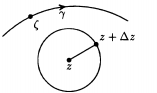
\includegraphics[scale=0.55]{pictures/ch34pict2}
        \caption{}
      \end{wrapfigure}
\item         Докажем формулу $\eqref{ch34eq6}$ при $n = 1$. Так как функция $q(\zeta)$ непрерывна на контуре $\gamma$, то существует число $M < + \infty$ такое, что $|q(\zeta)| \le M$ при $\zeta \in \gamma$.
      
Фиксируем точку $z \notin \gamma$. Пусть $d \triangleq \dist(z, \gamma)$. Очевидно, что $d > 0$. Выберем число $r \in (0, \frac{d}{2})$ и возьмем произвольное число $\Delta z \in \bbC$ так, чтобы $0 < |\Delta z| < r$. Тогда для $\forall \zeta \in \gamma$ получаем

\begin{equation} \label{ch34eq7}
|\zeta - (z + \Delta z)| \ge |\zeta - z| - |\Delta z| \ge d - \frac{d}{2} = \frac{d}{2}
\end{equation}

Оценим выражение }

\begin{equation} \label{ch34eq8}
\frac{I(z + \Delta z) - I(z)}{\Delta z} - \frac{1}{2 \pi i} \int_\gamma \frac{q(\zeta)}{(\zeta - z)^2}\,d\zeta = \frac{1}{2 \pi i} \int_\gamma q(\zeta) \left[ \left( \frac{1}{\zeta - z - \Delta z} - \frac{1}{\zeta - z} \right) \frac{1}{\Delta z} - \frac{1}{(\zeta - z)^2} \right] \,d\zeta.
\end{equation}

Упростим выражение в прямых скобках под интегралом $\eqref{ch34eq8}$:
\begin{multline*}
[\ldots] = \frac{{\zeta} - {z} - ({(\zeta} - {z}) - {\Delta z})}{(\zeta - z)((\zeta - z) - \Delta z)} \cdot \frac{1}{{\Delta z}} - \frac{1}{(\zeta - z)^2} = \frac{1}{(\zeta - z)(\Delta z- (\zeta-z) )} - \frac{1}{(\zeta - z)^2}=\\=
\frac{(\zeta - z)-(\Delta z- (\zeta-z))}{(\zeta - z)^2(\Delta z- (\zeta-z) )}
=\frac{\Delta z}{(\zeta - z)^2 (\zeta - z - \Delta z)} .
\end{multline*}
Поэтому для $\eqref{ch34eq8}$ получаем оценку 

$$
\left| \frac{\Delta I}{\Delta z} - \frac{1}{2\pi i} \int_\gamma \frac{q(\zeta)}{(\zeta - z)^2}\,d\zeta \right| 
\le \frac{1}{2\pi} \int_\gamma \frac{|q(\zeta)||\Delta z||\,d\zeta|}{|\zeta - z|^2|\zeta - z - \Delta z|}
\le \frac{|\Delta z|}{\pi d^3} \int_\gamma |q(\zeta)||\,d\zeta| 
\le \frac{|\Delta z| \cdot M}{\pi d^3} \int_\gamma |\,d\zeta| \xrightarrow{\Delta z \to 0} 0.
$$

Таким образом, в пределе получаем равенство

\begin{equation} \label{ch34eq9}
I'(z) = \frac{1}{2\pi i} \int_\gamma \frac{q(\zeta)}{(\zeta - z)^2} \,d\zeta.
\end{equation}

\item 
Общий случай $n$-й производной получается аналогично первому случаю из формулы $\eqref{ch34eq6}$ для $(n - 1)$-й производной и воспользовавшись биномом Ньютона

$$
(\zeta - z - \Delta z)^n = (\zeta - z)^2 - n \Delta z (\zeta - z)^{n - 1} + O(\Delta z^2),
$$

которое легко проверяется, например, методом математической индукции.
\end{enumerate}
\noindent
Теорема доказана.
\end{proof}

\begin{thm} \label{ch34Thm3}
Пусть функция $f : G \to \bbC$ регулярна в области $G \subset \bbC$. Тогда эта функция имеет в $G$ производные всех порядков, т.е. является бесконечно дифференцируемой функцией в области $G$.
\end{thm}

\begin{proof}
Фиксируем произвольную точку $z_0 \in G$, тогда существует число $r_0 > 0$ такое, что $\overline{B_{r_0}(z_0)}\subset G$. Пусть окружность $\gamma_{r_0} \triangleq \{ z \: \bigl| \: |z - z_0| = r_0 \}$ ориентирована положительно относительно внутренности круга (т.е. движением против хода часовой стрелки). Тогда по теореме \ref{ch34thm1} справедлива интегральная формула Коши

\begin{equation} \label{ch34eq10}
f(z) = \frac{1}{2\pi i} \int_{\gamma_{r_0}} \frac{f(\zeta)}{\zeta - z} \,d\zeta, \quad \forall z \in B_{r_0}(z_0).
\end{equation}

Так как формула $\eqref{ch34eq10}$ функция $\zeta \to f(\zeta)$ непрерывна на $\zeta_{r_0}$, то интеграл в $\eqref{ch34eq10}$ есть интеграл типа Коши, и по теореме \ref{ch34Thm2} он бесконечно дифференцируем в круге $B_{r_0}(z_0)$, т.е. в силу равенства $\eqref{ch34eq10}$ функция $f$ бесконечно дифференцируема в этом круге $B_{r_0}(z_0)$, при этом из $\eqref{ch34eq6}$ следует формула:

\begin{equation} \label{ch34eq11}
f^{n}(z) = \frac{n!}{2\pi i} \int_{\gamma_{r_0}} \frac{f(\zeta)}{(\zeta - z)^{n+1}}\,d\zeta, \quad \forall z \in B_{r_0}(z_0).
\end{equation}


Так как точка $z_0 \in G$ была произвольной, то функция $f$ бесконечно дифференцируема во всей области G.
\end{proof}


\section{Разложение функции, регулярной в окрестности точки, в ряд Тейлора}

Опираясь на интегральную формулу Коши, в этом параграфе покажем, что функция регулярна в окрестности некоторой точки тогда и только тогда, когда в этой окрестности она представима в виде суммы степенного ряда.

\begin{defn}
$\textit{Степенным рядом}$ называется функциональный ряд вида

\begin{equation} \label{ch34.2eq1}
\sum_{n = 0}^{+\infty}\limits c_n (z - a)^n,
\end{equation}
где точка $a \in \bbC$ и коэффициенты $c_n \in \bbC$ фиксированы.
\end{defn}

\begin{thm}[Абель] \label{ch34.2Thm1}
Если степенной ряд $\eqref{ch34.2eq1}$ сходится в точке $z_0 \not= a$, то ряд $\eqref{ch34.2eq1}$ сходится абсолютно в любой точке из круга $B_{|z_0 - a|}(a)$, а в любом замкнутом круге $\overline{B_{r}(a)}$, где $0 < r < |z_0 - a|$, этот ряд сходится равномерно.
\end{thm}

\begin{proof}\leavevmode
\addpicture[6]{pictures/ch34pict3}{0.3}

Так как по условию числовой ряд $\sum_{n = 0}^{+\infty}\limits c_n (z - a)^n$ сходится, то из необходимого условия сходимости рядов следует, что $\lim\limits_{n \to \infty} |c_n(z_0 - a)^n| = 0$, поэтому существует число $\alpha > 0$ такое, что $|c_n(z_0 - a)^n| \le \alpha$ для всех $n$.
\begin{enumerate}
\item[1)] \rightskip=3.5cm { Пусть точка $z \in B_{|z_0 - a|}(a)$. Тогда $|c_n(z_0 - a)^n| = |c_n(z_0 - a)^n \cdot \left| \frac{z - a}{z_0 - a} \right|^n \le \alpha q^{n}_z$, где $q_z \triangleq \left| \frac{z - a}{z_0 - a} \right| < 1$. Так как числовой ряд $\sum_{n = 0}^{\infty}\limits q_{z}^n$ очевидно сходится, то по признаку сравнения ряд $\eqref{ch34.2eq1}$ сходится и абсолютно в точке $z$.
}
\item[2)] \rightskip=0cm Определим $q_0 \triangleq \frac{r}{|z_0 - a|}\ge\left|\frac{z - a}{z_0 - a}\right|$. Аналогично пункту 1 получаем оценку: $|c_n(z - a)^n| \le \alpha q^{n}_0$. Так как числовой ряд $\sum_{n = 0}^{\infty}\limits q_{0}^n$ очевидно сходится, то по признаку Вейештрасса(см. ниже) ряд $\eqref{ch34.2eq1}$ сходится равномерно на круге $\overline{B_{r}(a)}$.
\end{enumerate}
\rightskip=-3.3cm Теорема доказана.
\end{proof}

\begin{stt}[Признак Вейерштрасса]
Пусть $|f_n(z)| \le a_n$ для $\forall n \in \bbN$ и $\forall z \in G$ и пусть числовой ряд $\sum\limits_{n = 0}^{+\infty} a_n$ сходится. Тогда функциональный ряд $\sum_{n = 0}^{+\infty}\limits f_n(z)$ сходится абсолютно и равномерно на $G$. 
\end{stt}

Эта теорема \ref{ch34.2Thm1} позволяет получить представление об области сходимости степенного ряда $\eqref{ch34.2eq1}$.

Определим для степенного ряда $\eqref{ch34.2eq1}$ понятие $\textit{радиуса сходимости}$:

\begin{equation} \label{ch34.2eq2}
R \triangleq \sup \{ |z - a| \: \big| \: \sum_{n = 0}^{+\infty} c_n (z - a)^n \: \text{сходится} \}.
\end{equation}

Тогда, если $0 < R < +\infty$, то в силу теоремы \ref{ch34.2Thm1} Абеля в каждой точке круга $B_R(a)$ ряд $\eqref{ch34.2eq1}$ сходится, а в каждой точке $z \notin \overline{B_R(a)}$ ряд $\eqref{ch34.2eq1}$ расходится. Круг $B_R(a)$ называется кругом сходимости ряда $\eqref{ch34.2eq1}$.
Радиус сходимости $R$ степенного ряда $\eqref{ch34.2eq1}$ может быть вычислен по известной формуле Коши-Адамара (причем, в ней не исключено $R=\pm\infty$):

\begin{equation} \label{ch34.2eq3}
R = \frac{1}{\overline{\lim\limits_{n \to \infty}} \sqrt[n]{|c_n|}}
\end{equation}

\begin{exmpl} \label{exmpl2}
Ряд вида $\sum\limits_{n = 0}^{+\infty} z^n$, являющийся суммой бесконечной геометрической прогрессии, очевидно сходится при $|z| < 1$ к функции $\frac{1}{1 - z}$, так как легко посчитать, что

$$
S_N(z) \triangleq \sum\limits_{n = 0}^{N} z^n = \left( \sum\limits_{n = 0}^{N} z^n \right) \frac{1 - z}{1 - z} =\frac{1-z+z-\dots-z^N+z^N-z^{N+1}}{1-z}= \frac{1 - z^{N + 1}}{1 - z}  \xrightarrow{N \to \infty} \frac{1}{1 - z}.
$$

\end{exmpl} 
\begin{stt} \label{ch34stt1000}
Пусть в области $G$ заданы непрерывные функции $f_n: G \to \bbC, \: n \in \bbN$ и кусочно-гладкий контур $\gamma$. Пусть функциональный ряд $\sum\limits_{n = 0}^{+\infty}f_n(z)$ сходится к своей сумме $S(z)$ равномерно на контуре $\gamma$. Тогда этот ряд можно почленно интегрировать по контуру $\gamma$, т.е. справедливо равенство 

\begin{equation} \label{ch34eq1000} 
\int\limits_{\gamma}S(z) \,dz = \sum\limits_{n = 0}^{+\infty} \int\limits_{\gamma} f_n(z) \,dz. 
\end{equation} 

\end{stt}
\begin{defn}
Пусть у функции $f : B_r(a) \to \bbC$ существуют в точке $a \in \bbC$, $r > 0$, производные $f^{(n)}(a)$ любого порядка $n \in \bbN$. Тогда степенной ряд вида

\begin{equation} \label{ch34.2eq4}
\sum\limits_{n = 0}^{+\infty} \frac{f^{(n)}(a)}{n!} (z - a)^n
\end{equation}
называется $\textit{рядом Тейлора функции f}$ с центром в точке $a$.
\end{defn}

\begin{thm}\leavevmode
Если функция $f$ регулярна в круге $B_r(a)$, где $a \in \bbC$, $r > 0$, то она представима в этом\addpicture[6]{pictures/ch34pict4.png}{0.4}\label{ch34pict4} \noindent  круге $B_r(a)$ в виде суммы сходящегося ряда Тейлора, т.е.

\begin{equation} \label{ch34.2eq5}
f(z) = \sum\limits_{n = 0}^{\infty} c_n(z - a)^n, \quad \forall z \in B_r(a),
\end{equation}

где

\begin{equation} \label{ch34.2eq6}
c_n = \frac{f^{(n)}(a)}{n!}.
\end{equation}

\end{thm}

\begin{proof}
Фиксируем произвольную точку $z \in B_r(a)$. Тогда существует число $r_1 > 0$ такое, что $|z - a| < r_1 < r$.

Пусть $\gamma_{r_1} \triangleq \{\zeta \: \big| \: |\zeta - a| = r_1 \}$ — ориентированная движением против хода часовой стрелки окружность (см. рис. \ref{ch34pict4}). Запишем интегральную формулу Коши:

\begin{equation} \label{ch34.2eq7}
f(z) = \frac{1}{2 \pi i} \int_{\gamma_{r_1}} \frac{f(\zeta)}{\zeta - z} \,d\zeta.
\end{equation}

Преобразуем функцию $\zeta \to \frac{1}{\zeta - z}$, где $\zeta \in \gamma_{r_1}$, к виду

$$
\frac{1}{\zeta - z} = \frac{1}{(\zeta - a) - (z - a)} = \frac{1}{(\zeta - a)\left( 1 - \frac{z - a}{\zeta - a}\right)}.
$$
Здесь $\left|\frac{z - a}{\zeta - a} \right| = \frac{|z - a|}{r_1} \triangleq q, q < 1$. Как в примере $\ref{exmpl2}$, получаем разложение в сходящийся ряд

$$
\frac{1}{\zeta - z} = \frac{1}{\zeta - a} \left( 1 + \frac{z - a}{\zeta - a} + \left( \frac{z - a}{\zeta - a}\right)^2 + \ldots \right) = \sum\limits_{n = 0}^{+\infty} \frac{(z - a)^n}{(\zeta - a)^{n + 1}}.
$$
В итоге, подынтегральная функция в $\eqref{ch34.2eq7}$ представима сходящимся на $\gamma_{r_1}$ рядом

\begin{equation} \label{ch34.2eq8}
\frac{f(\zeta)}{\zeta - z} = \sum\limits_{n = 0}^{+\infty} \frac{(z - a)^n}{(\zeta - a)^{n + 1}} f(\zeta), \quad \forall \zeta \in \gamma_{r_1}.
\end{equation}

Так как справедлива оценка

$$
\left| \frac{(z - a)^n}{(\zeta - a)^{n + 1}} f(\zeta) \right| \le \frac{M}{r_1} \cdot q^n, \quad \text{где} \quad M = \sup_{\zeta \in \gamma_{r_1}} |f(\zeta)| < +\infty,
$$
а ряд $\sum\limits_{n = 0}^{\infty} q^n$ сходится, то по признаку Вейерштрасса функциональный ряд $\eqref{ch34.2eq8}$ сходится равномерно на окружности $\gamma_{r_1}$. Поэтому в силу утверждения \ref{ch34stt1000} ряд $\eqref{ch34.2eq8}$ можно почленно интегрировать по окружности $\gamma_{r_1}$. В результате получаем равенство

\begin{equation} \label{ch34.2eq9}
f(z) = \sum\limits_{n = 0}^{\infty} \frac{1}{2\pi i} \int_{\gamma_{r_1}} \frac{f(\zeta)}{(\zeta - a)^{n + 1}} \,d\zeta \cdot (z - a)^n,
\end{equation}
т.е. степенной ряд вида $\eqref{ch34.2eq1}$ с коэффициентами

\begin{equation} \label{ch34.2eq10}
c_n = \frac{1}{2\pi i} \int_{\gamma_{r_1}} \frac{f(\zeta)}{(\zeta - a)^{n + 1}} \,d\zeta.
\end{equation}
Эти коэффициенты $c_n$ не зависят от выбора точки $z$ или окружности $\gamma_{r_1}$, так как, воспользовавшись формулой для производной для интеграла типа Коши, получаем для $c_n$ формулу $\eqref{ch34.2eq6}$. Таким образом, ряд $\eqref{ch34.2eq9}$ есть ряд Тейлора функции $f$. В силу произвольности $z \in B_r(a)$ ряд $\eqref{ch34.2eq9}$ сходится в круге $B_r(a)$, а поэтому его радиус сходимости $R \ge r$.
\end{proof}

\begin{cons} \label{cons1}
Пусть функция $f$ регулярна в области $G$ и пусть выбрана точка $a \in G$. Тогда функция $f$ представима в виде ряда Тейлора

$$
f(z) = \sum\limits_{n = 0}^{+\infty} \frac{f^{(n)}(a)}{n!} (z - a)^n,
$$
который сходится по крайней мере в круге $B_R(a)$ максимального радиуса $R > 0$, при котором этот круг содержится в области $G$ (см. рис. 2).

\end{cons}